\section{Results and discussion}\label{Sec:Results}
 
The results presented in this section include the transverse momentum spectra, integrated yields, \myield, and mean transverse momentum, \mpt, as a function of \SOPT, as well as \pt-differential ratios between particle species (mainly with respect to pions), and the \pt-differential ratios-to-\PI relative to the \SOPT unbiased baseline (referred to as the ``double ratio''). Finally, the strangeness enhancement as a function of \SOPT is investigated.



In the following, the \myield and \mpt are calculated in the measured kinematic range, and corrected for the limited range by extrapolating the spectra to the unmeasured \pt regions using Levy--Tsallis fits down to \pt = 0. To account for the additional systematic uncertainties arising from this procedure, modified fit functions such as Boltzmann, $m_{\rm T}$-exponential, \pt-exponential, Fermi-Dirac (only for fermions) and Bose--Einstein statistics (only for bosons), and Boltzmann--Gibbs blast-wave functions are used as variations. The systematic uncertainties arising due to extrapolations are evaluated from the RMS of the variations with respect to the Levy--Tsallis fits. The extrapolation uncertainty is added in quadrature to the systematic uncertainties obtained from the measured \pt ranges to get the final systematic uncertainties for the \myield and \mpt. More details about this procedure can be found in Ref.~\cite{alice_newstrangeness}.


The experimental measurements will be compared with a broad selection of \pp MC models, namely PYTHIA 8.2~\cite{Torbjorn} (both the default Monash tune and with the added rope hadronization framework), Herwig 7.2~\cite{Herwig}, and EPOS-LHC~\cite{EPOS-LHC}. PYTHIA 8.2 is a QCD-inspired model that is built around the Lund-string model for hadronization~\cite{pythia8}. The default Monash tune is unable to describe the strangeness enhancement in small systems, while the rope extension (layers of overlapping strings that increase the string tension) of the Lund-string model~\cite{Ropes} has been introduced to accommodate this. For the PYTHIA 8.2 Ropes, note that this article only utilizes the "Flavour Ropes" for the model predictions, without the string-shoving mechanism~\cite{Bierlich:2016vgw} incorporated in the rope hadronization framework. Similarly, Herwig is a QCD-inspired \pp generator centered around a cluster hadronization model~\cite{Herwig}, which has recently been extended to be able to describe the strangeness enhancement~\cite{ALICE:2020nkc}. On the contrary, EPOS-LHC is a two-component core-corona model, which incorporates QGP features in the core to explain the strangeness enhancement.


The effect of the \SOPT selection is discussed in Sec.~\ref{Sec:ResHM} for the two multiplicity estimators. It is shown that the spherocity selection for the events with the highest midrapidity multiplicity, 0--1\% \tracklet, gives the best control of the event ``hardness'', i.e. select events with a large \mpt. Results obtained using this estimator are therefore first presented in Secs.~\ref{Sec:ResSpec}--~\ref{Sec:IntYield}, followed by results obtained using other multiplicity estimators in Sec.~\ref{Sec:ResExpMult}.

\subsection{High-multiplicity estimators and \SOPT}\label{Sec:ResHM}

If one considers a high-multiplicity \pp collision to be built up from independent subcollisions (a traditional MPI picture~\cite{MPI}), then there will be a trivial isotropization with increasing multiplicity. As previous ALICE measurements indicate a strong correlation between multiplicity and QGP-like effects, such as strangeness production~\cite{Naturepaper}, it is important for the study presented here to disentangle this possible trivial bias from the underlying physical properties of interest. To understand the impact of this on the \SOPT selection, the \mpt and the average pion yield $\langle \rm{d}\it{N}_{\pi}/\rm{d}\it{y} \rangle$, with different multiplicity and spherocity selection criteria are shown in Fig.~\ref{Fig:CL1vsV0M}. Results are shown for both the forward (V0M) and midrapidity (\tracklet) multiplicity estimators (described in Sec.~\ref{Sec:Mult}). A clear distinction is observed with respect to how the different multiplicity estimators relate to the \SOPT selection. This effect is solely driven by the rapidity region where the multiplicity is estimated, and not by properties of the ALICE apparatus.

\begin{figure}[h!]
    \centering
    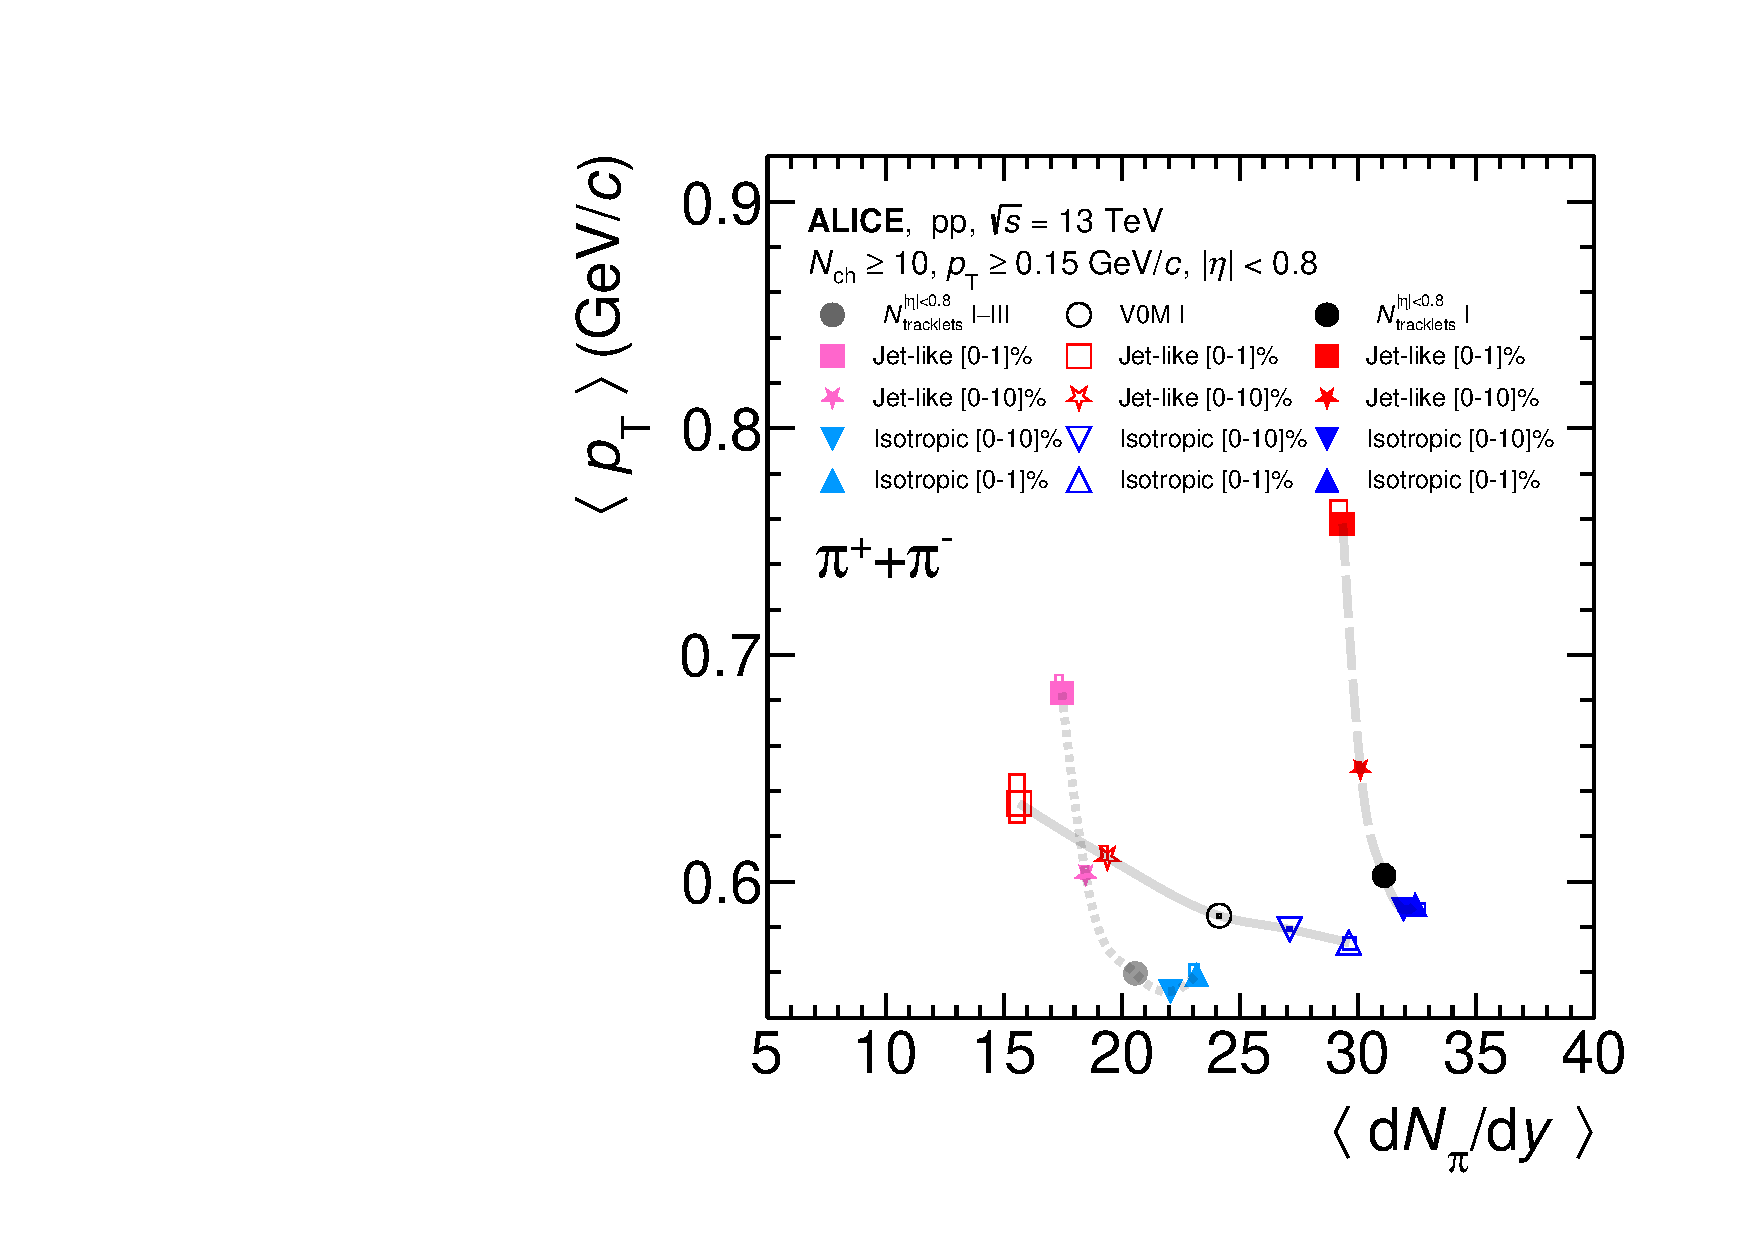
\includegraphics[scale=0.6]{figures/mgPion_0.pdf}
    \caption{Correlation between $\langle p_{\rm{T}}\rangle$ and $\langle \rm{d}N_{\pi}/\rm{d}y \rangle$ as a function of \SOPT, in the 0--10\% and 0--1\% V0M and \tracklet multiplicity classes. The total systematic uncertainties are represented by empty boxes. The statistical uncertainty is smaller than the reported marker sizes.}
    \label{Fig:CL1vsV0M}
\end{figure}

It is observed that the V0M multiplicity selection maintains a similar \mpt, but contains large variations in \myieldpi for the different \SOPT selections. In contrast, the \tracklet selected events are characterized by large differences in \mpt among the event classes, selecting events according to their hardness. The implicit multiplicity dependence of \SOPT is minimized by sharply constraining the multiplicity using a midrapidity multiplicity estimation. This implies that the \tracklet multiplicity estimator, in tandem with a \SOPT selection, is best at separating events based on their hardness.

Moreover, PYTHIA 8.2 model studies of the correlation between the average transverse momentum transfer of the hardest parton--parton interaction, $\left<\pthat\right>$, and the average number of multi-parton interactions $\left<n\textrm{MPI}\right>$ is presented in Fig.~\ref{Fig:pthatvsmpi} for multiplicity and \SOPT intervals of 0--1\%. For each estimator, the multiplicity is calculated as the number of primary charged particles in the pseudorapidity interval(s) covered by that estimator. Figure~\ref{Fig:pthatvsmpi} shows that the hardest scattering for the events in the jet-like \SOPT 0--1\% event category is significantly harder than for the \SOPT-integrated, high-multiplicity reference. This is observed both for the default PYTHIA 8.2 Monash, and with the rope hadronization framework enabled. This feature is present when the multiplicity is estimated both in the \tracklet and V0M pseudorapidity regions, but the effect is particularly strong when the multiplicity is estimated at midrapidity. Furthermore, the isotropic \SOPT 99--100\% events are slightly softer than overall high-multiplicity events. In conjunction with the softer \mpt presented in Fig.~\ref{Fig:CL1vsV0M}, these findings suggest that the isotropic topologies are formed by multiple softer interactions, while the jet-like topologies have at least one hard scattering that is significantly harder than for the \SOPT-integrated selection.


\begin{figure}[h!]
    \centering
    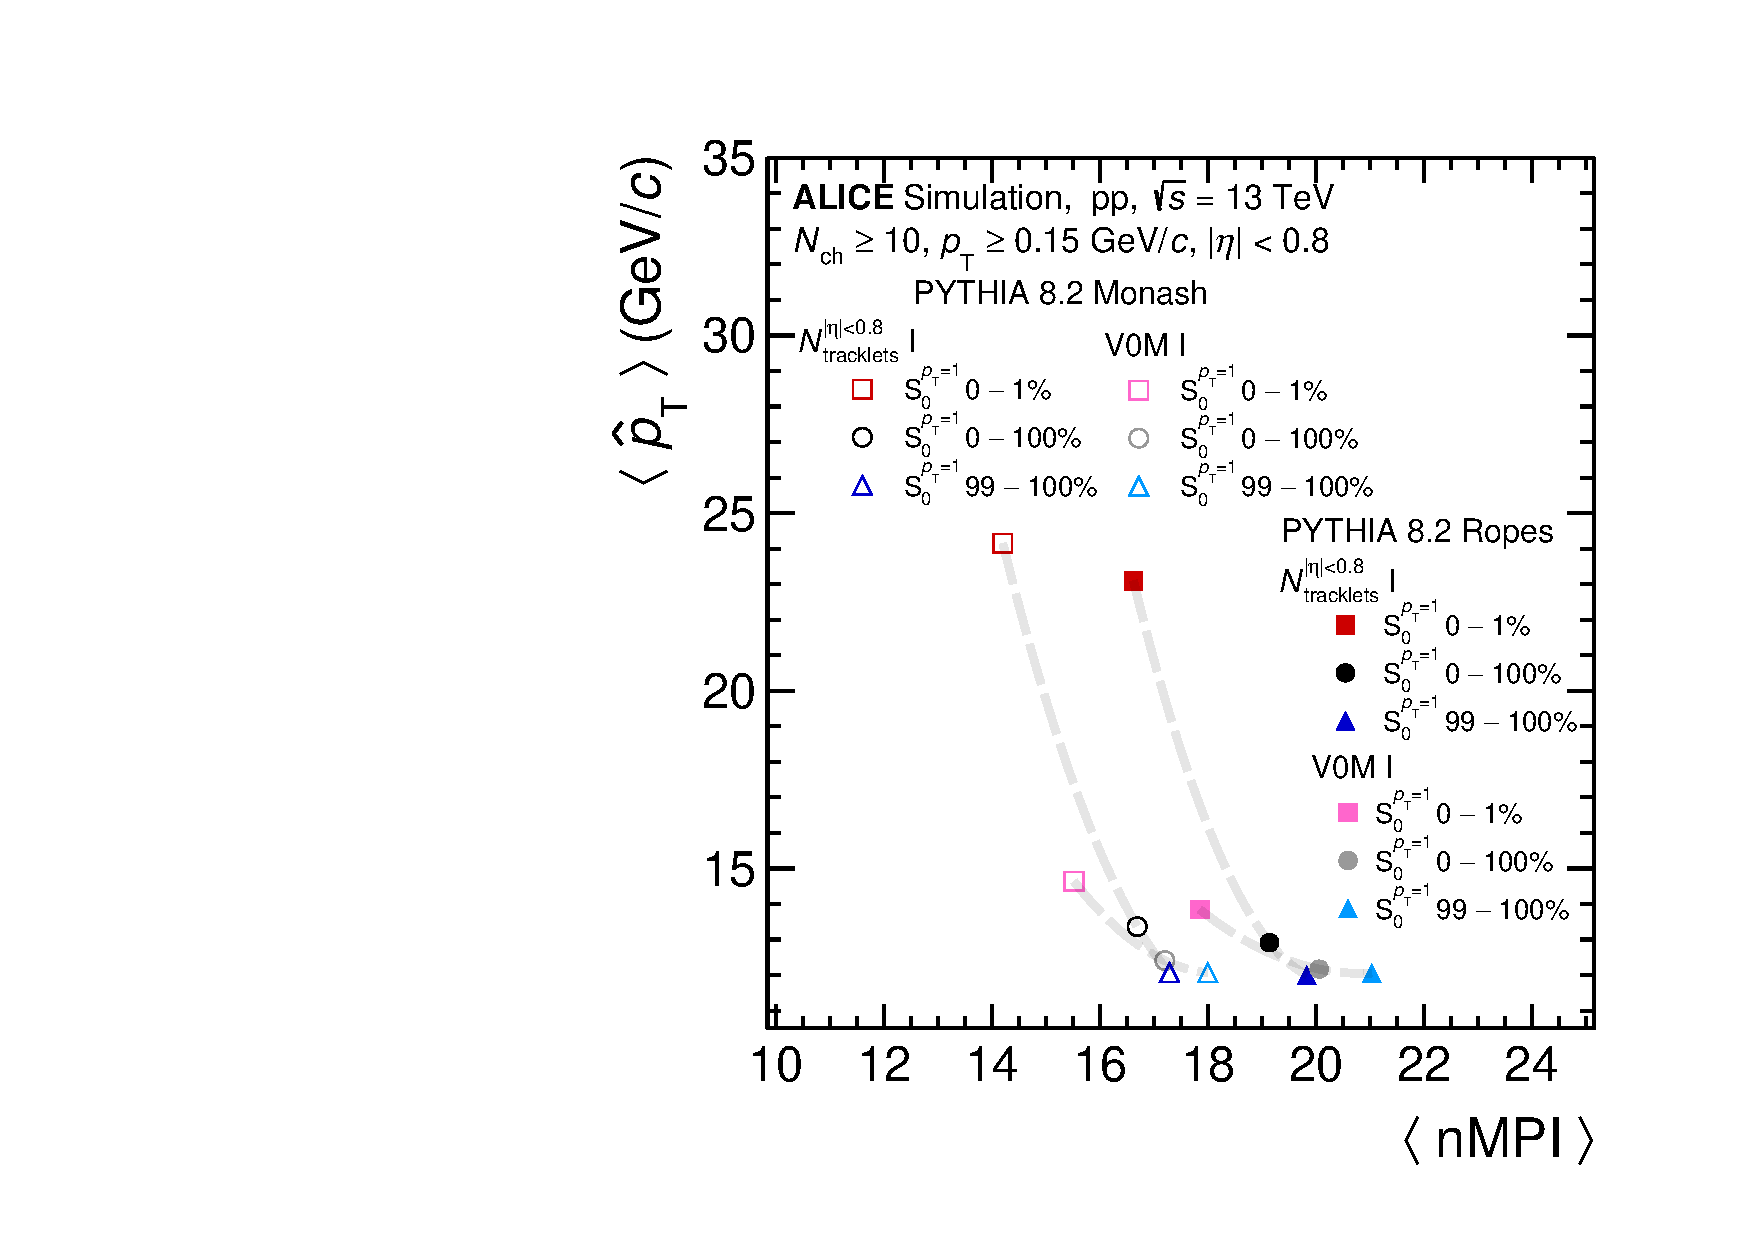
\includegraphics[scale=0.6]{figures/pthat_vs_nmpi.pdf}
    \caption{PYTHIA 8.2 correlation study between $\left<\pthat\right>$ and $\left<n\textrm{MPI}\right>$ as a function of \SOPT, in 0--1\% V0M and \tracklet multiplicity classes. The default PYTHIA 8.2 Monash variation is compared to PYTHIA 8.2 with color rope hadronization. The total systematic and statistical uncertainties are smaller than the marker sizes. The grey band is an interpolation between the points, to more clearly illustrate the trend of each multiplicity and model variation.}
    \label{Fig:pthatvsmpi}
\end{figure}
In the following, a complete set of results will be presented using \tracklet 0--1\% to highlight the impact on the QCD dynamics of the extreme event topologies, while minimizing the effects of any trivial multiplicity (system size) dependence. The results are first presented for jet-like and isotropic events, utilizing a 0--10\% and 90--100\% \SOPT selection, respectively, to have a complete set of particle spectra. Furthermore, selected results are also presented for the most extreme 1\% percentiles of \SOPT. 
